
\begin{columns}[t]
	\begin{column} {0.32\textwidth}
		\begin{block}{\large Data Collection}
			\centering
				\vspace{0.2in}
				\begin{figure}[h]
					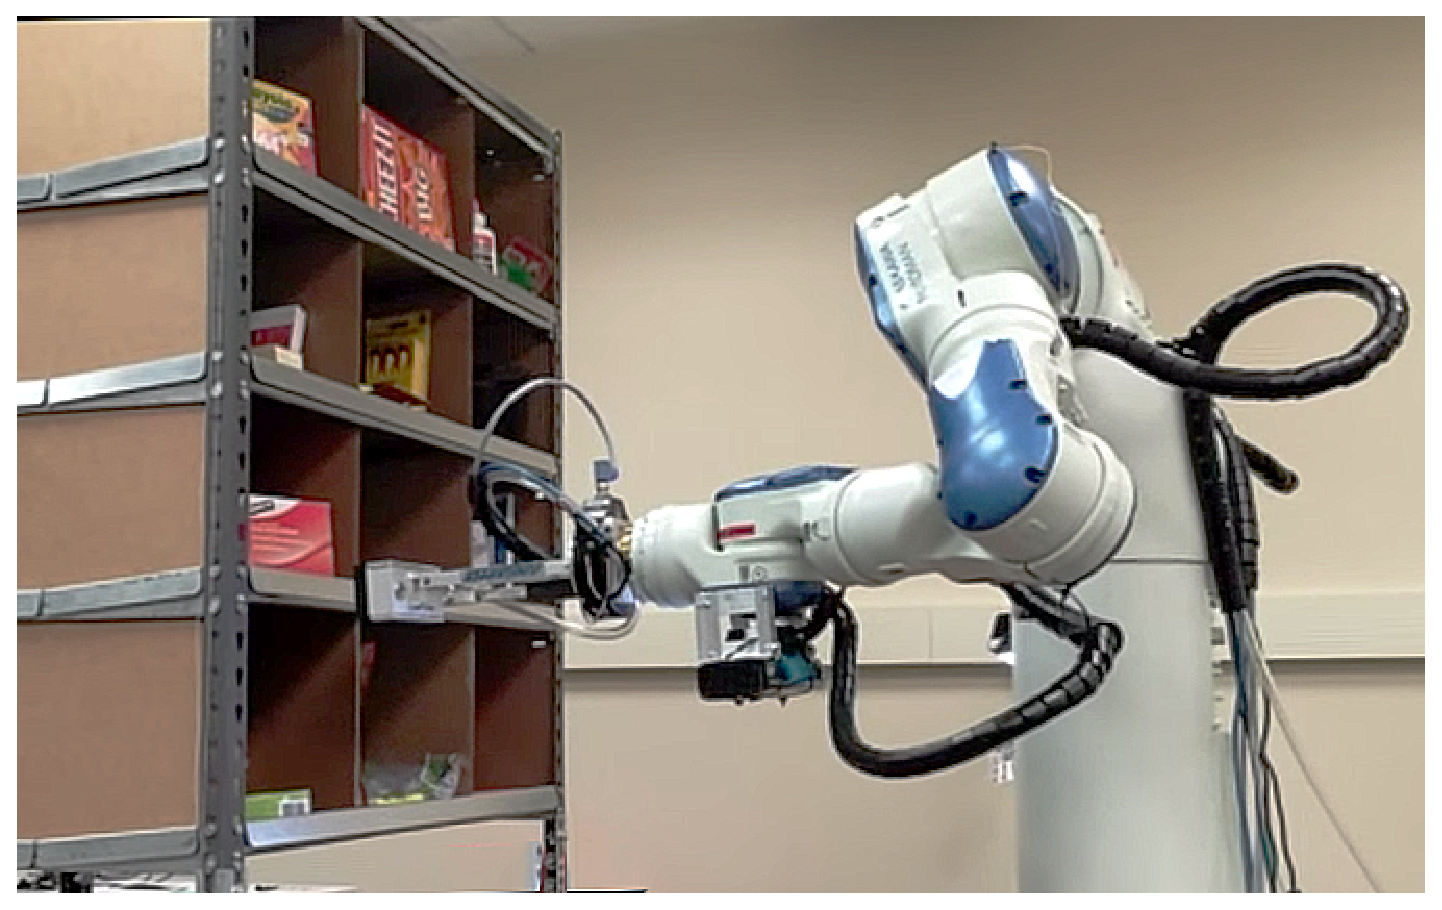
\includegraphics[width=0.8\textwidth]{datacollectionsetup_2}
					\caption{Our data collection hardware and environment}
				\end{figure}
				% \vspace{0.1in}
					\begin{columns}[t]
						\begin{column}{0.94\textwidth}
							\begin{itemize}
								\item Collection performed on Motoman Dual-arm SDA10F humanoid robot using Kinect v1 RGBD camera
								\item Camera located on wrist of robot, position calibrated prior to data collection
								\item 10,368 RGBD images collected involving 24 target objects, each shown in:
									\begin{itemize}
										\item 12 different bin locations
										\item 3 clutter states per bin (1, 2, 3 items)
										\item 3 viewpoints per clutter state
										\item 4 frames per viewpoint
									\end{itemize}
								\item 6D Ground truth annotated by hand, including all transformations between object, camera, and robot base
							\end{itemize}
						\end{column}
					\end{columns}
				\vspace{0.1in}
		\end{block}
		% \begin{block}{\large Monotone Method by Stilman et al. '07}
		% 	\begin{itemize}
		% 		\item Adaptation of previous work for solving rearrangement tasks.
		% 		\item Backtracking search for monotone problems.
		% 		\item Computationally fast even upon failure.
		% 		\item Requirement: no overlapping initial and target poses. 			 
		% 	\end{itemize}
		% 	\centering
		% 	% \includegraphics [width=0.43\blocklen] {monotone1} \hspace {0.5in}
		% 	% \includegraphics [width=0.43\blocklen] {monotone2}
		% \end{block}
	\end{column}
	%Second general Column
	\begin{column}{0.68\textwidth}
		\begin{block} {\large Dataset Features}
			\begin{columns}[T]
				\centering
				\begin{column}{0.59\textwidth}
					\begin{itemize}
						\item Large dataset covering wide variety of objects with 6D ground truth object pose annotatations
						\item Good sample coverage of probable object poses within the shelves
						\item Provides researchers the ability to determine the effects of immediate clutter on pose estimation
							\begin{itemize}
								\item Same ground truth target object pose is given with varying degrees of clutter within the bin
							\end{itemize}
						\item Allows opportunity to analyze accuracy based on the camera's viewpoint
							\begin{itemize}
								\item For each shelf configuration, samples are generated from 3 different viewing positions
							\end{itemize}
						\item Provides the ability to determine the effects of slight sensor noise on deterministic algorithms
							\begin{itemize}
								\item For each shelf configuration at each viewpoint 4 samples are generated
							\end{itemize}
					\end{itemize}
					
				\end{column}
				\begin{column}{0.40\textwidth}
					\centering
					\begin{figure}[h]
						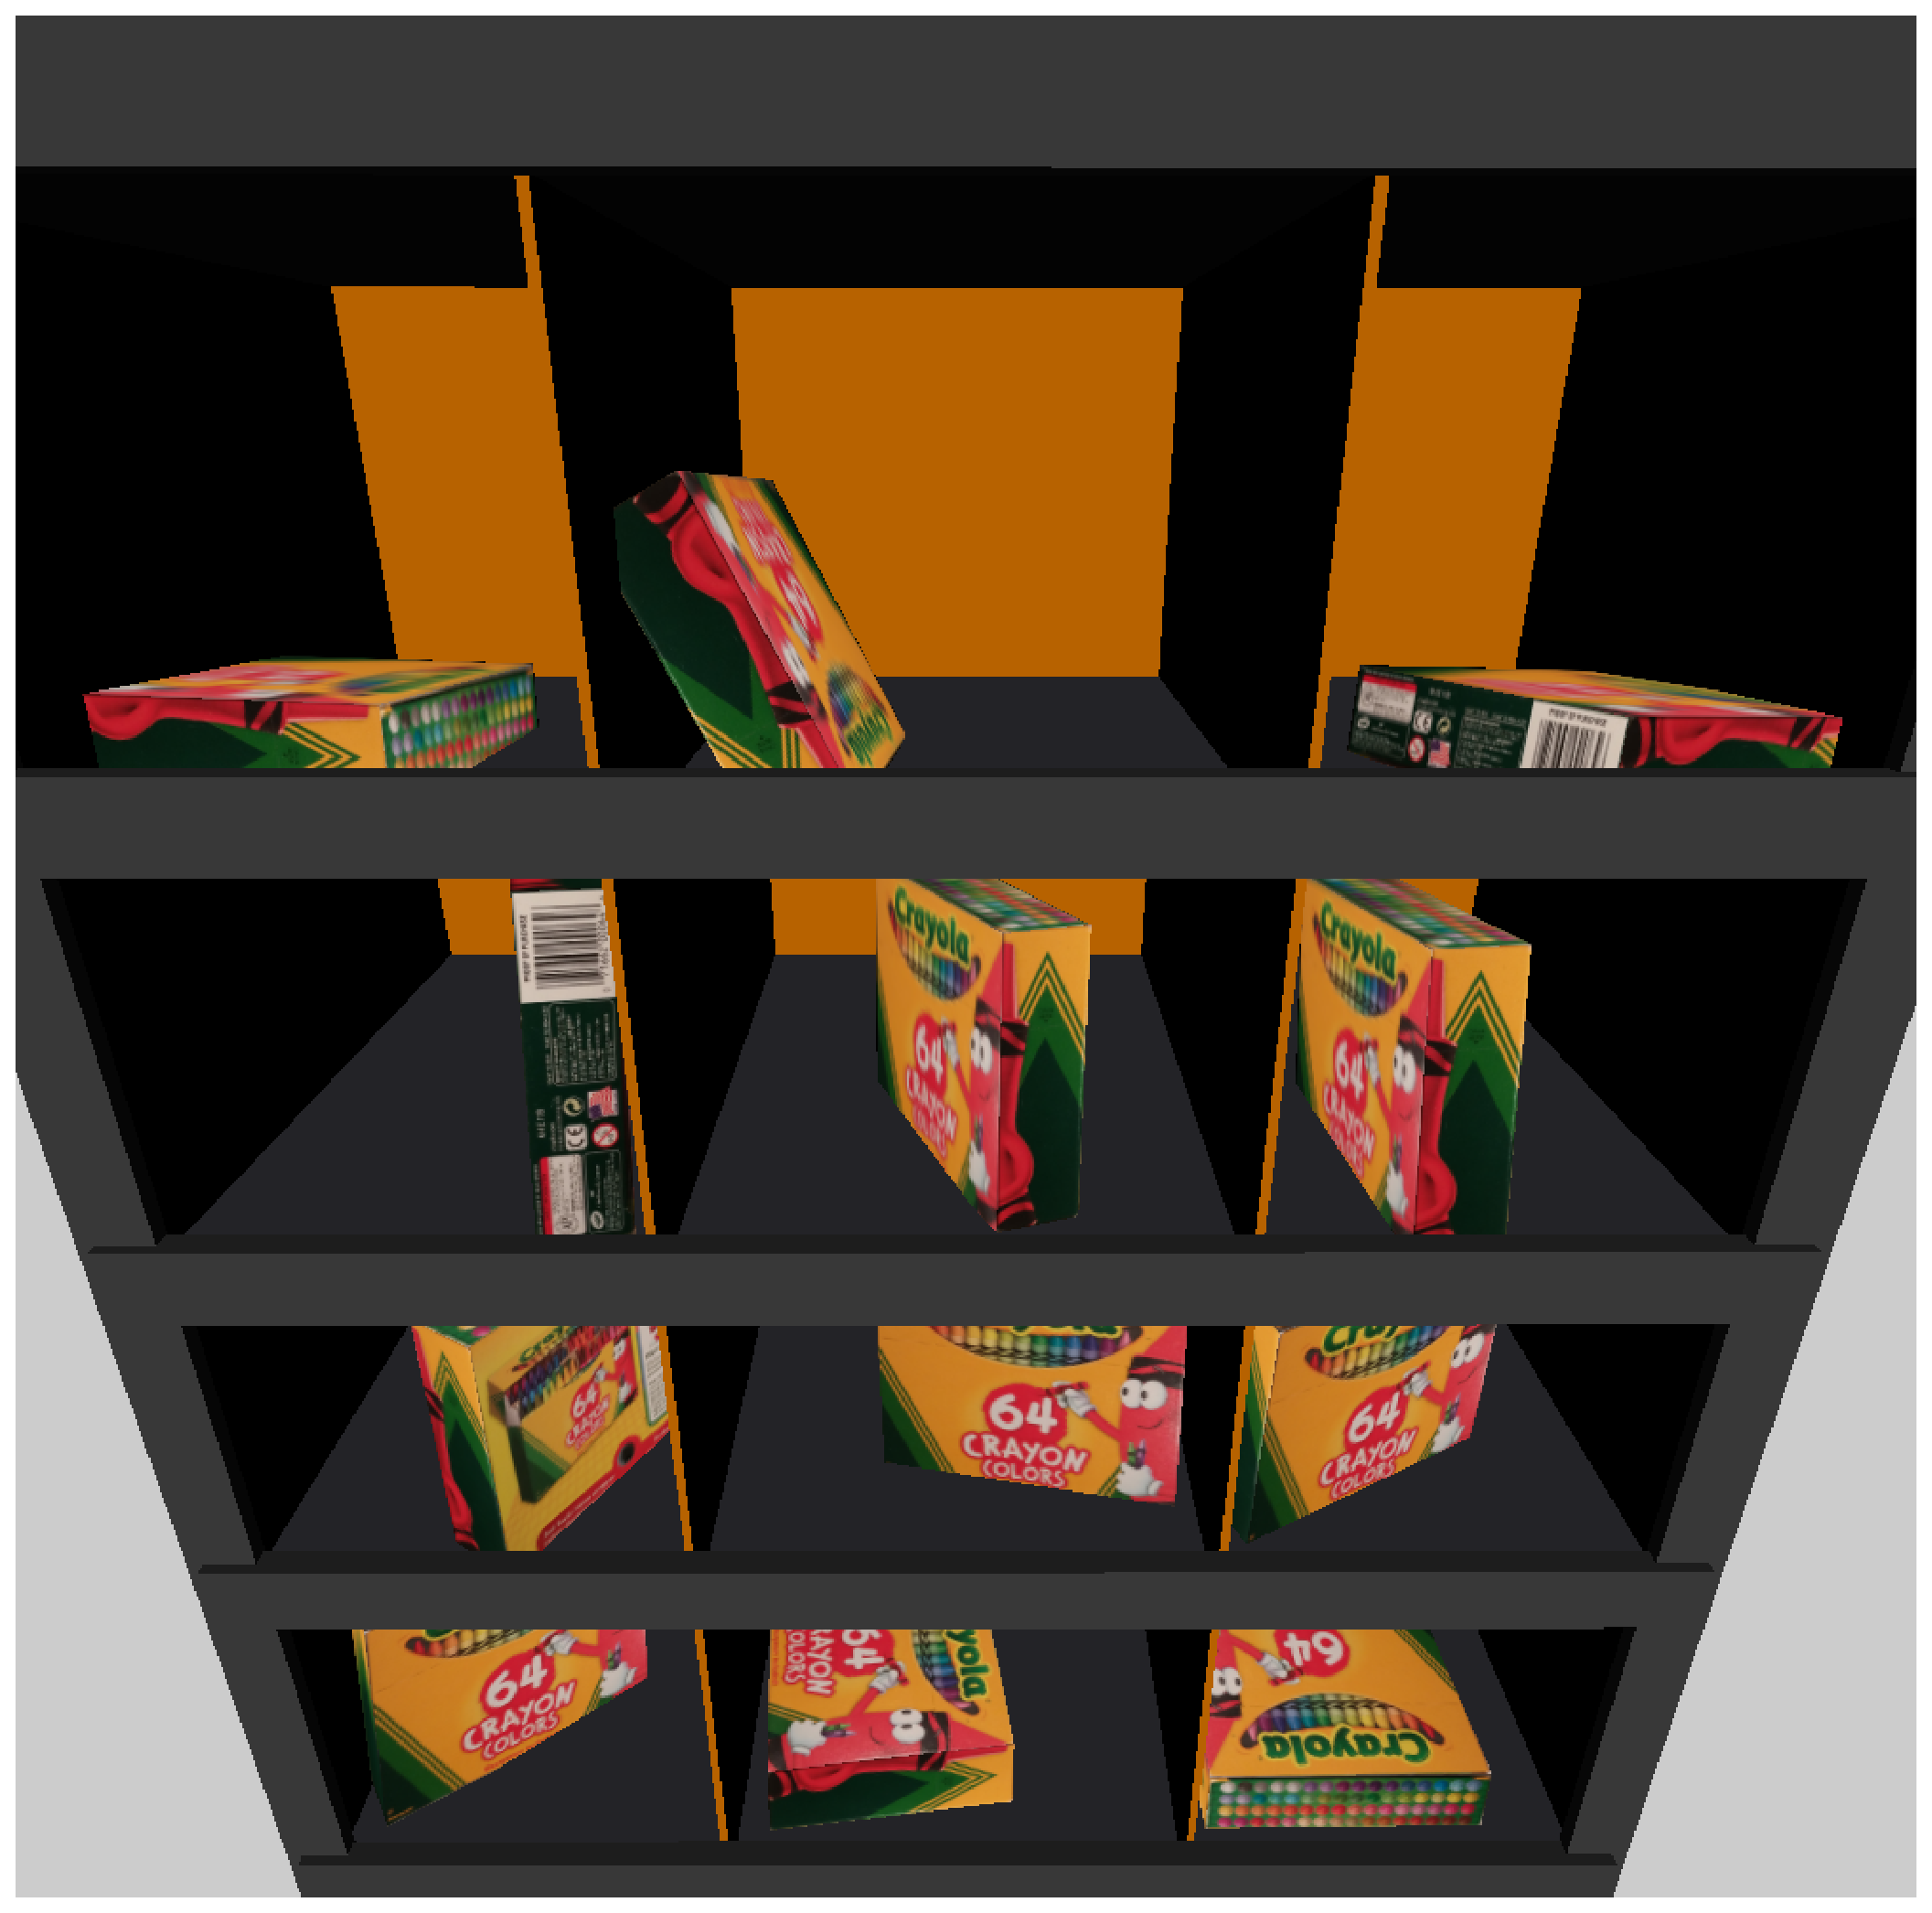
\includegraphics[width=0.8\textwidth]{shelf_positions}
						\caption{Variety of coverage in our dataset of ground truth poses for a single object}
					\end{figure}
				\end{column}
			\end{columns}
			\hspace{0.02\textwidth}
			\begin{figure}[h]
				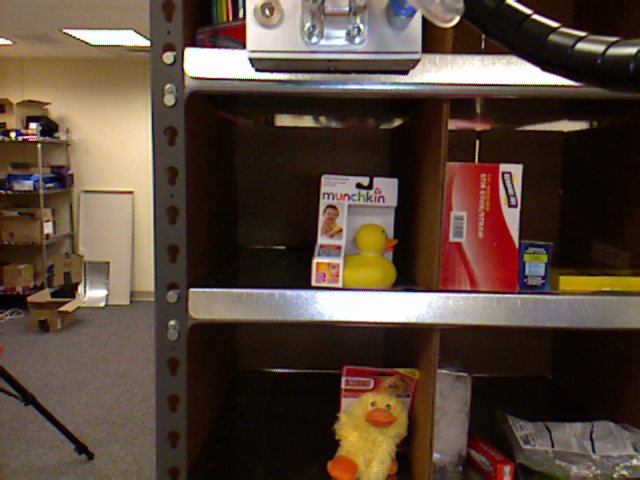
\includegraphics[width=0.3\textwidth]{munchkin_1} \hspace{0.02\textwidth}
				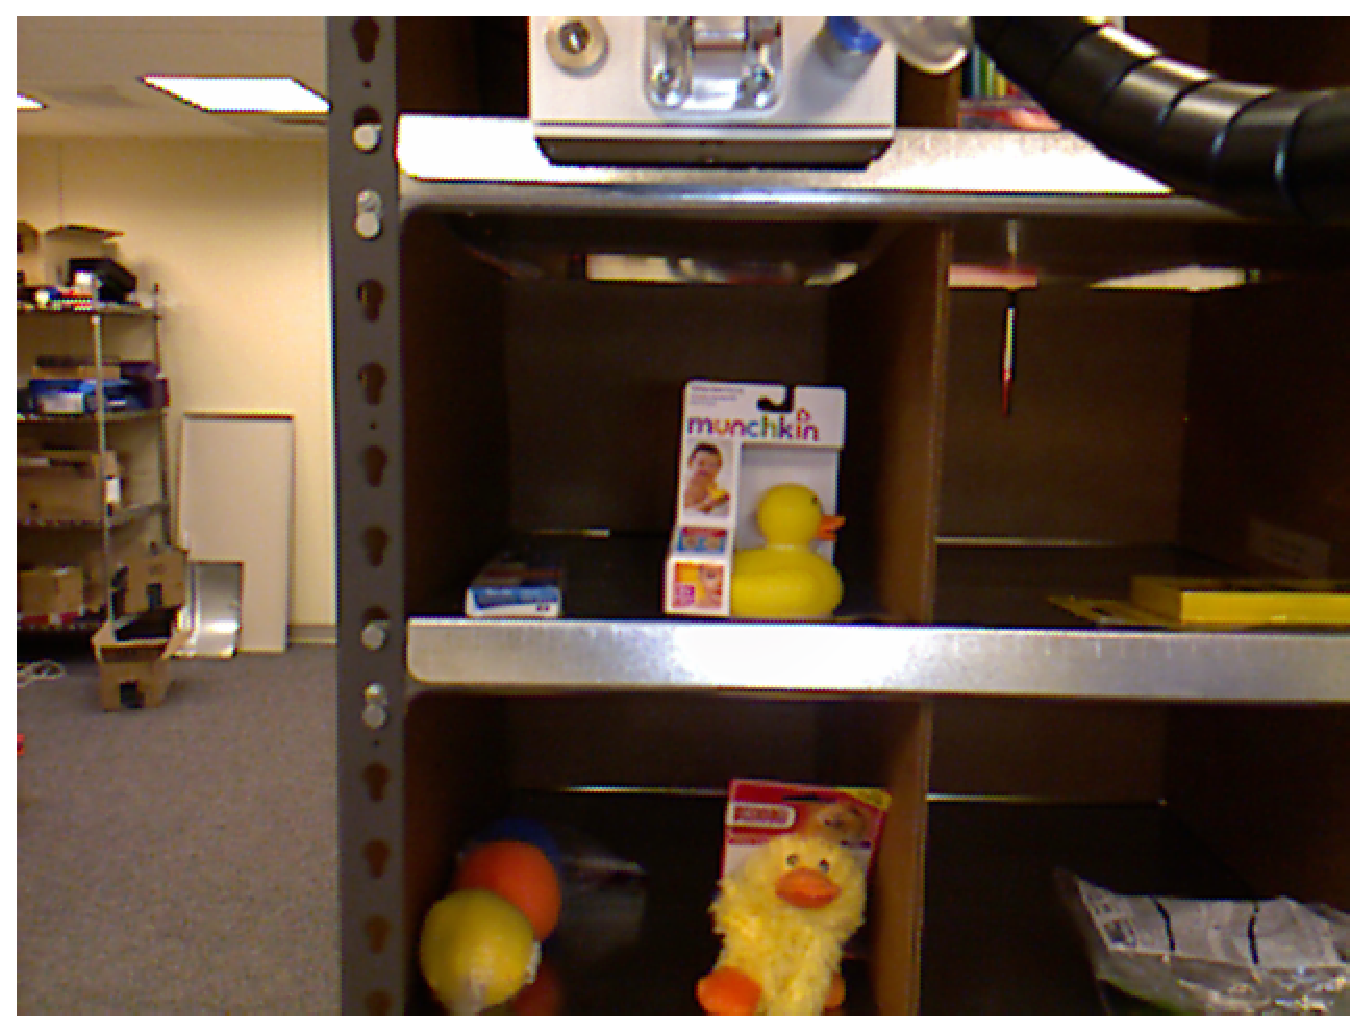
\includegraphics[width=0.3\textwidth]{munchkin_2} \hspace{0.02\textwidth}
				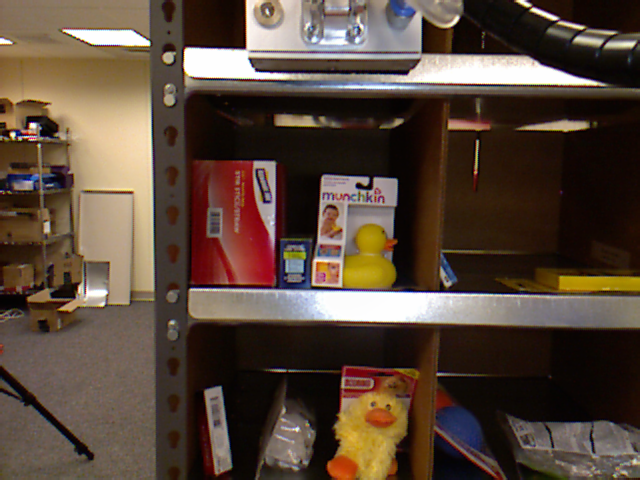
\includegraphics[width=0.3\textwidth]{munchkin_3} 
				\caption{Examples from our dataset showing the same target object pose (the ``duck'') in varying degrees of clutter within the bin}
			\end{figure}
		\end{block}
		% \begin{block}{\large Non-monotone Extension}
		% 	\begin{itemize}
		% 		\item Evacuate the blocking objects to intermediate poses. 
		% 		\item Solve Minimum Constraint Removal Problem to detect intermediate poses.
		% 		\item Requirement: Enough space to move blocking objects.
		% 	\end{itemize}
		% 	\begin{columns}[T]
		% 		\begin{column}{0.48\blocklen}
		% 			\centering
		% 			% \includegraphics [width=0.45\blocklen] {nonmonotone1}
		% 			{\small
		% 			\begin{itemize}
		% 				\item The method works regardless the order with which objects are evacuated.
		% 			\end{itemize}
		% 			}
		% 		\end{column}
		% 		\begin{column}{0.48\blocklen}
		% 			\centering
		% 			% \includegraphics [width=0.45\blocklen] {nonmonotone2}
		% 			{\small
		% 			\begin{itemize}
		% 				\item Backward search for detecting a valid sequence of objects evacuations.  
		% 			\end{itemize}
		% 			}
		% 		\end{column}
		% 	\end{columns}
		% \end{block}
	\end{column}
\end{columns}



